\documentclass{standalone}
\usepackage{tikz}
\usetikzlibrary{patterns, positioning}


\begin{document}
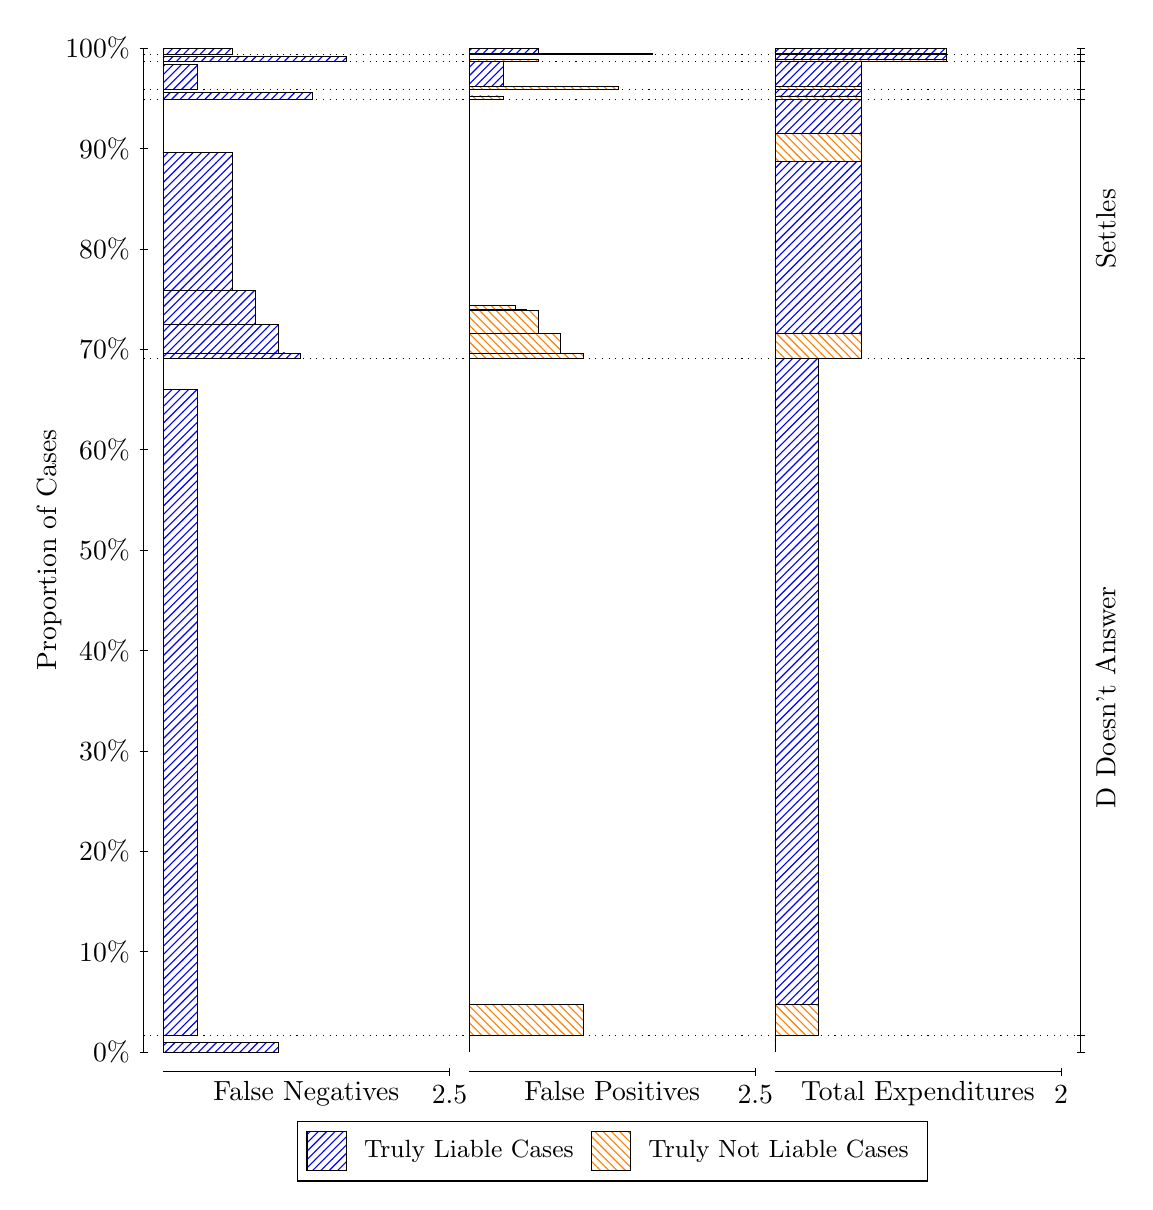
\begin{tikzpicture}
\draw[black, very thin] (1.5,1.75) -- (1.5,14.5);
\node[rotate=90, text=black, anchor=center] at (0.3, 8.125) {Proportion of Cases};
\draw[black, very thin] (1.45,1.75) -- (1.55,1.75);
\node[text=black, anchor=east] at (1.45, 1.75) {0\%};
\draw[black, very thin] (1.45,3.025) -- (1.55,3.025);
\node[text=black, anchor=east] at (1.45, 3.025) {10\%};
\draw[black, very thin] (1.45,4.3) -- (1.55,4.3);
\node[text=black, anchor=east] at (1.45, 4.3) {20\%};
\draw[black, very thin] (1.45,5.575) -- (1.55,5.575);
\node[text=black, anchor=east] at (1.45, 5.575) {30\%};
\draw[black, very thin] (1.45,6.85) -- (1.55,6.85);
\node[text=black, anchor=east] at (1.45, 6.85) {40\%};
\draw[black, very thin] (1.45,8.125) -- (1.55,8.125);
\node[text=black, anchor=east] at (1.45, 8.125) {50\%};
\draw[black, very thin] (1.45,9.4) -- (1.55,9.4);
\node[text=black, anchor=east] at (1.45, 9.4) {60\%};
\draw[black, very thin] (1.45,10.675) -- (1.55,10.675);
\node[text=black, anchor=east] at (1.45, 10.675) {70\%};
\draw[black, very thin] (1.45,11.95) -- (1.55,11.95);
\node[text=black, anchor=east] at (1.45, 11.95) {80\%};
\draw[black, very thin] (1.45,13.225) -- (1.55,13.225);
\node[text=black, anchor=east] at (1.45, 13.225) {90\%};
\draw[black, very thin] (1.45,14.5) -- (1.55,14.5);
\node[text=black, anchor=east] at (1.45, 14.5) {100\%};

\draw[black, very thin] (13.4,1.75) -- (13.4,14.5);
\draw[black, very thin] (13.35,1.75) -- (13.45,1.75);
\node[anchor=west] at (13.35, 1.75) {};
\draw[black, very thin] (13.35,1.9584) -- (13.45,1.9584);
\node[anchor=west] at (13.35, 1.9584) {};
\draw[black, very thin] (13.35,10.555) -- (13.45,10.555);
\node[anchor=west] at (13.35, 10.555) {};
\draw[black, very thin] (13.35,13.851) -- (13.45,13.851);
\node[anchor=west] at (13.35, 13.851) {};
\draw[black, very thin] (13.35,13.977) -- (13.45,13.977);
\node[anchor=west] at (13.35, 13.977) {};
\draw[black, very thin] (13.35,14.329) -- (13.45,14.329);
\node[anchor=west] at (13.35, 14.329) {};
\draw[black, very thin] (13.35,14.42) -- (13.45,14.42);
\node[anchor=west] at (13.35, 14.42) {};
\draw[black, very thin] (13.35,14.5) -- (13.45,14.5);
\node[anchor=west] at (13.35, 14.5) {};

\draw[black, very thin, pattern color=blue, pattern=north east lines] (1.75,1.75) rectangle (3.2033,1.8678);
\draw[black, very thin, pattern color=orange, pattern=north west lines] (1.75,1.8678) rectangle (1.75,1.9584);
\draw[black, very thin, pattern color=blue, pattern=north east lines] (1.75,1.9584) rectangle (2.186,10.163);
\draw[black, very thin, pattern color=orange, pattern=north west lines] (1.75,10.163) rectangle (1.75,10.555);
\draw[black, very thin, pattern color=blue, pattern=north east lines] (1.75,10.555) rectangle (3.494,10.618);
\draw[black, very thin, pattern color=blue, pattern=north east lines] (1.75,10.618) rectangle (3.3487,10.627);
\draw[black, very thin, pattern color=blue, pattern=north east lines] (1.75,10.627) rectangle (3.2033,10.988);
\draw[black, very thin, pattern color=blue, pattern=north east lines] (1.75,10.988) rectangle (2.9127,11.421);
\draw[black, very thin, pattern color=blue, pattern=north east lines] (1.75,11.421) rectangle (2.622,13.171);
\draw[black, very thin, pattern color=orange, pattern=north west lines] (1.75,13.171) rectangle (1.75,13.851);
\draw[black, very thin, pattern color=blue, pattern=north east lines] (1.75,13.851) rectangle (3.6393,13.938);
\draw[black, very thin, pattern color=orange, pattern=north west lines] (1.75,13.938) rectangle (1.75,13.977);
\draw[black, very thin, pattern color=blue, pattern=north east lines] (1.75,13.977) rectangle (2.186,14.29);
\draw[black, very thin, pattern color=orange, pattern=north west lines] (1.75,14.29) rectangle (1.75,14.329);
\draw[black, very thin, pattern color=blue, pattern=north east lines] (1.75,14.329) rectangle (4.0753,14.394);
\draw[black, very thin, pattern color=orange, pattern=north west lines] (1.75,14.394) rectangle (1.75,14.42);
\draw[black, very thin, pattern color=blue, pattern=north east lines] (1.75,14.42) rectangle (2.622,14.493);
\draw[black, very thin, pattern color=orange, pattern=north west lines] (1.75,14.493) rectangle (1.75,14.5);
\draw[black, very thin, pattern color=orange, pattern=north west lines] (5.6333,1.75) rectangle (5.6333,1.8406);
\draw[black, very thin, pattern color=blue, pattern=north east lines] (5.6333,1.8406) rectangle (5.6333,1.9584);
\draw[black, very thin, pattern color=orange, pattern=north west lines] (5.6333,1.9584) rectangle (7.0867,2.351);
\draw[black, very thin, pattern color=blue, pattern=north east lines] (5.6333,2.351) rectangle (5.6333,10.555);
\draw[black, very thin, pattern color=orange, pattern=north west lines] (5.6333,10.555) rectangle (7.0867,10.619);
\draw[black, very thin, pattern color=orange, pattern=north west lines] (5.6333,10.619) rectangle (6.796,10.876);
\draw[black, very thin, pattern color=orange, pattern=north west lines] (5.6333,10.876) rectangle (6.5053,11.171);
\draw[black, very thin, pattern color=orange, pattern=north west lines] (5.6333,11.171) rectangle (6.36,11.176);
\draw[black, very thin, pattern color=orange, pattern=north west lines] (5.6333,11.176) rectangle (6.2147,11.235);
\draw[black, very thin, pattern color=blue, pattern=north east lines] (5.6333,11.235) rectangle (5.6333,13.851);
\draw[black, very thin, pattern color=orange, pattern=north west lines] (5.6333,13.851) rectangle (6.0693,13.891);
\draw[black, very thin, pattern color=blue, pattern=north east lines] (5.6333,13.891) rectangle (5.6333,13.977);
\draw[black, very thin, pattern color=orange, pattern=north west lines] (5.6333,13.977) rectangle (7.5227,14.016);
\draw[black, very thin, pattern color=blue, pattern=north east lines] (5.6333,14.016) rectangle (6.0693,14.329);
\draw[black, very thin, pattern color=orange, pattern=north west lines] (5.6333,14.329) rectangle (6.5053,14.355);
\draw[black, very thin, pattern color=blue, pattern=north east lines] (5.6333,14.355) rectangle (5.6333,14.42);
\draw[black, very thin, pattern color=orange, pattern=north west lines] (5.6333,14.42) rectangle (7.9587,14.428);
\draw[black, very thin, pattern color=blue, pattern=north east lines] (5.6333,14.428) rectangle (6.5053,14.5);
\draw[black, very thin, pattern color=orange, pattern=north west lines] (9.5167,1.75) rectangle (9.5167,1.8406);
\draw[black, very thin, pattern color=blue, pattern=north east lines] (9.5167,1.8406) rectangle (9.5167,1.9584);
\draw[black, very thin, pattern color=orange, pattern=north west lines] (9.5167,1.9584) rectangle (10.062,2.351);
\draw[black, very thin, pattern color=blue, pattern=north east lines] (9.5167,2.351) rectangle (10.062,10.555);
\draw[black, very thin, pattern color=orange, pattern=north west lines] (9.5167,10.555) rectangle (10.607,10.876);
\draw[black, very thin, pattern color=blue, pattern=north east lines] (9.5167,10.876) rectangle (10.607,13.059);
\draw[black, very thin, pattern color=orange, pattern=north west lines] (9.5167,13.059) rectangle (10.607,13.418);
\draw[black, very thin, pattern color=blue, pattern=north east lines] (9.5167,13.418) rectangle (10.607,13.851);
\draw[black, very thin, pattern color=orange, pattern=north west lines] (9.5167,13.851) rectangle (10.607,13.891);
\draw[black, very thin, pattern color=blue, pattern=north east lines] (9.5167,13.891) rectangle (10.607,13.977);
\draw[black, very thin, pattern color=orange, pattern=north west lines] (9.5167,13.977) rectangle (10.607,14.016);
\draw[black, very thin, pattern color=blue, pattern=north east lines] (9.5167,14.016) rectangle (10.607,14.329);
\draw[black, very thin, pattern color=orange, pattern=north west lines] (9.5167,14.329) rectangle (11.697,14.355);
\draw[black, very thin, pattern color=blue, pattern=north east lines] (9.5167,14.355) rectangle (11.697,14.42);
\draw[black, very thin, pattern color=orange, pattern=north west lines] (9.5167,14.42) rectangle (11.697,14.428);
\draw[black, very thin, pattern color=blue, pattern=north east lines] (9.5167,14.428) rectangle (11.697,14.5);
\draw[black, dotted] (1.5,1.9584) -- (13.4,1.9584);
\draw[black, dotted] (1.5,10.555) -- (13.4,10.555);
\draw[black, dotted] (1.5,13.851) -- (13.4,13.851);
\draw[black, dotted] (1.5,13.977) -- (13.4,13.977);
\draw[black, dotted] (1.5,14.329) -- (13.4,14.329);
\draw[black, dotted] (1.5,14.42) -- (13.4,14.42);
\draw[black, very thin] (1.75,1.5) -- (5.3833,1.5);
\node[text=black, anchor=north] at (3.5667, 1.5) {False Negatives};
\draw[black, very thin] (5.3833,1.45) -- (5.3833,1.55);
\node[text=black, anchor=north] at (5.3833, 1.45) {2.5};

\draw[black, very thin] (5.6333,1.5) -- (9.2667,1.5);
\node[text=black, anchor=north] at (7.45, 1.5) {False Positives};
\draw[black, very thin] (9.2667,1.45) -- (9.2667,1.55);
\node[text=black, anchor=north] at (9.2667, 1.45) {2.5};

\draw[black, very thin] (9.5167,1.5) -- (13.15,1.5);
\node[text=black, anchor=north] at (11.333, 1.5) {Total Expenditures};
\draw[black, very thin] (13.15,1.45) -- (13.15,1.55);
\node[text=black, anchor=north] at (13.15, 1.45) {2};


\node[text=black, centered, rotate=90] at (13.72, 6.2568) {D Doesn't Answer};
\node[text=black, centered, rotate=90] at (13.72, 12.203) {Settles};





\draw (7.449999999999999,1.5) node[draw=none] (baseCoordinate) {};
\begin{scope}[align=center]
        \matrix[scale=0.5, draw=black, below=0.5cm of baseCoordinate, nodes={draw}, column sep=0.1cm]{
            \node[rectangle, draw, minimum width=0.5cm, minimum height=0.5cm, pattern color=blue, pattern=north east lines] {}; &
            \node[draw=none, font=\small, text=black] (B) {Truly Liable Cases}; &
            \node[rectangle, draw, minimum width=0.5cm, minimum height=0.5cm, pattern color=orange, pattern=north west lines] {}; &
            \node[draw=none, font=\small, text=black] (B) {Truly Not Liable Cases}; \\
            };
\end{scope}

\end{tikzpicture}
\end{document}